% !TEX root = ../../report.tex

\section{Generating implicit ratings}

As discussed in Section~\ref{implicit-feedback} we can generate ratings based
on observed user behaviours in order to create a better experience for the
users, by not asking them to explicitly rate items. Hence, by having robust
methods for generating (implicit) ratings based on these logs we can create
common recommender systems models and recommend items without the user actively
taking part of the process.

\ref{levels-frequency}
\subsection{Levels of frequency, with global popularity}

Considering the weaknesses presented in Section~\ref{levels-frequency}, namely
choosing good weights and only using a small percentage of the scale between
0-100. Further, the method presented does not differentiate between active and
less active users, thus ignoring the entropy once the maximal level is reached.
Instead we extend the method by considering the global popularity of each item,
so that the user that.. \marginpar{Finish the subsection about improving leveled
freq}

\subsection{Introduction to the sigmoid-function}

Extending our models further we want to capture our intuition that recent
events should count more towards a good rating, compared to old events. We
differentiate between two ways of classifying an event $e_u$ as old or recent;
one where we count the number of days between the newest event $e_n$ and event
$e_u$; and the second where we count the number of other events between $e_n$
and $e_u$. However, intuitively we consider a user to have multiple relevant
items concurrently and we know that in domains such as technology, fashion and
other consumer-products an item has an ago of relevancy, somewhat metaphoric to
a seasonal threshold. An example of this could be a fashion store recommending
warm clothes in the months between December to March, but then want to "change"
product pool based on the users behaviours – who are probably looking for
lighter clothes (changing season).

By considering recentness we also implicitly add negative feedback to events,
as in practice we are penalizing the ratings for old events. This is an
important aspect to keep in mind when working with implicit feedback, as
discussed in Section~\ref{implicit-feedback} as modern recommender engines work
better when we are assuming ratings are based on both positive and negative
feedback.

In order to catch our intuition mathematically we use a logistic function, which
is a mathematical function having an "S" shape and a common special case of the
more general sigmoid-function. In its most simplest case the logistic function
is defined as:

% Vertical alignment of equation and plot.
\begin{figure}[H]
  \centering
  \noindent\begin{minipage}{.45\textwidth}
    \begin{tikzpicture}
      \begin{axis}
      \addplot[black,xlabel=$x$,ylabel=$f(x)$] {1/(1+exp(-x))};
      \end{axis}
    \end{tikzpicture}
  \end{minipage}
  \begin{minipage}{.45\textwidth}
  \begin{align}
    \label{logistic-function}
    f(x) = \frac{1}{1+\exp^{-x}}
  \end{align}
  \end{minipage}
  \caption{Logistic function having a S-shape with y-values ranging
  from 0 to 1.}
\end{figure}

Here the value of $f(x)$ is asymptotically limited between 0 and 1, dependent
on the value of $x$. The steepest point of the curve happens when $x=0$. By
adjusting the exponent of $e^{(-x)}$ we can skew the curve in order to map to our
data, giving us a \textit{function of relevancy} ranging from an item being
very relevant ($f(x)=0$) and not relevant ($f(x)=1$).

By adding two variables to the logistic function we can fine tune both the
steepness and range of $f(x)$. Hence we adjust Equation~\ref{logistic-function}
to include $s$, the \textit{steepness coefficient}, and $r$, the \textit{shift
coefficient}. By default these are $1$ and $0$ respectively, but by adjusting
$s$ closer to 0 we decrease the steepness, creating a more gradual curve.
Setting the $r$ to a larger number we shift the steepest point of the curve to
$x=r$, hence if we set $r$ to $20$, the steepest point (largest acceleration)
in our curve would be located when $x=20$.
\marginpar{show equation using these coefficients}

\subsection{Considering number of days since event}

In order to better understand the usage of the logistic function, we consider
an example event log.
%We are considering the following event log for user $u$ on product $p$, where
%our goal is to give a implicit rating based on different event types and the
%number of days between events.

\begin{table}[H]
  \centering
  \label{events-example}
  \begin{tabular}{p{4cm}m{3cm}}
    \toprule
    Number of days since most recent event & Unique event types \\
    \midrule
    5 & 1,2,3 \\
    10 & 1 \\
    15 & 1,2 \\
    \bottomrule
  \end{tabular}
\end{table}

As discussed in Section~\ref{implicit-feedback} and
Section~\ref{levels-frequency} we will use levels of frequency to order or
event types by scores, or rather importance. But, instead of sampling scores
between a given range we use a interval start and stop value - and use the
whole range of float values in this interval as possible scores. We can
imagine, for the purpose of this example that we have the following score
intervals:

\begin{table}[H]
  \centering
  \label{implicit-example-scores}
  \begin{tabular}{lll}
    \toprule
    Event type & Min. score & Max. score \\
    \midrule
    1 & 20 & 60 \\
    2 & 60 & 80 \\
    3 & 80 & 100 \\
    \bottomrule
  \end{tabular}
  \caption{Example of a scoring scheme using continious scores between a min.
  and max value as possible implicit scores}
\end{table}

\marginpar{\textbf{todo}: do evaluation on different schemes}
As discussed earlier, the way we assign these scores is at the moment fairly
naive, some results using various schemes are given in Section~\ref{}. The main
thing to note is that we use non-overlapping intervals in order to do various
optimizations in our algorithms and also that the interval for the most common
event (typically a product click or similar) is $3x$ as big as our higher
valued event types. This is done in order to create a larger differentiation
of scores between events of same type in the same time space.

Using the events in Table~\ref{events-example} we set our shift coefficient $r$
to $14.0$, and the steepness coefficient $s$ to $0.4$ in order to both match
our domain specific goals (short life span of products and seasonal activity)
and get a good spread in final ratings as our dataset is small. This yields the
following logistic function:

\begin{figure}[h!]
  \centering
  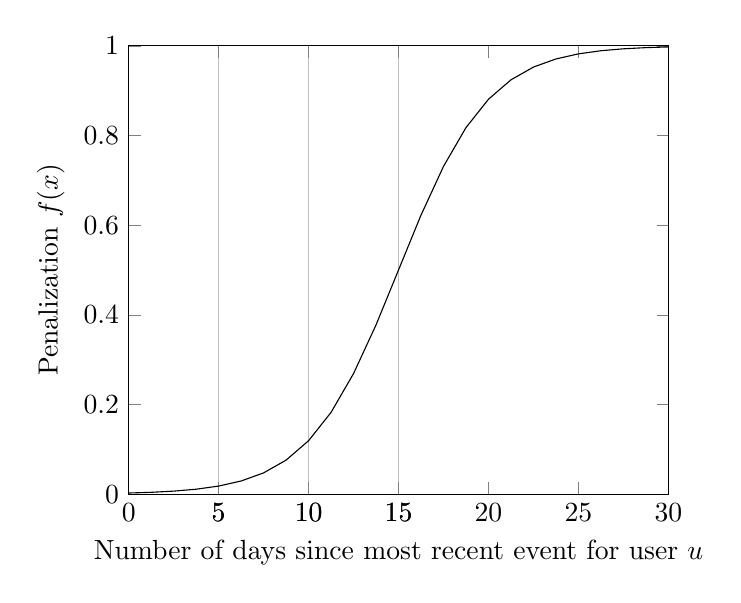
\begin{tikzpicture}
    \begin{axis}[
      ymin=0,ymax=1,
      xmin=0,xmax=30,
      xlabel=Number of days since most recent event for user $u$,
      ylabel=Penalization $f(x)$,
      extra x ticks={5,10,15},
      extra tick style={grid=major}
    ]
    \addplot[
    black,
    xlabel=$x$,
    ylabel=$f(x)$,
    domain=0:30]
    {1/(1+exp(-0.4*(x-15)))};
    \end{axis}
  \end{tikzpicture}
\end{figure}

As one can see, an event happening 15 days after the most recent event for user
$u$ will get a penalization of $0.5$ whilst an event with $x=5$ recieves
$0.018$. Following up on Table~\ref{events-example} we can calculate the
various penalizations and final scores for each day, by taking the highest
possible score for event $i$ and penalizing it in the following manner:

\begin{equation}
  s_{e}(x,u) = b_e - (b_e - w_e) \cdot p_{x}(u)
\end{equation}

where $p_x$ is the penalization after $x$ days. $b_e$ and $w_e$ are the best
and worst scores achievable for event $e$, respectivly. The final score
$s_{e}(x,u)$ is presented for each event below:

\begin{table}[H]
  \centering
  \label{events-example}
  \begin{tabular}{llm{2cm}ll}
    \toprule
    Num. days ($x$) & Event types & Penalization $p_{x}(u)$ & Scores & Highest score \\
    \midrule
    5   & 1,2,3 & 0.018   & 59.1, 79.64, 99.64 & \textbf{99.64} \\
    10  & 1     & 0.1192  & 55.23              & 55.23  \\
    15  & 1,2   & 0.5     & 50.0, 70.0         & 70.0 \\
    \bottomrule
  \end{tabular}
\end{table}
\marginpar{Perhaps represent this differently?}

When selecting a score for user $u$ we select the highest valued one, in this
case 99.64. In fact, we can optimize our algorithm by starting at the most
recent events and not calculating scores for events types that yield a lower
score than the current highest score. In the scenario above we could take all
events on $x=5$, then taken the event type with highest maximum value (3) and
ignored all other events. Note that this is only true if you have
non-overlapping event type scores/intervals, as we have per
Table~\ref{implicit-example-scores}. We can now normalize $s$ and get a rating
$r$ between $a$ and $b$ by using the following equation, knowing that $X_{max}
= 100$ and $X_{min} = 0$:

\begin{equation}
  \label{eq-normalization}
  X' = a + \frac{(X-X_{min})\cdot(b-a)}{X_{max}-X_{min}}
\end{equation}

Setting $a$ to 0 and $b$ to 5, as is common in recommender systems we get the
rating $X' = 4.982$ when $s = 99.64$. Intuitivly this makes sense, if we assume
event type 3 to be the highest valued event in our system it would be
equivalaent to a user buying a product - or similar. Thus, if user $u$ bought
product $i$ only $5$ days ago this would get $4.98$ as final rating. If the
user does not interact with the product again in 30 days we can re-calculate
the score, now using $x=35$ which yields a penalization of $0.999$ and score $s
= 100-((100-80)*0,999) = 80.2$, normalized in the same likert scale as above we
get a new normalized rating $4.01$ - thus still a high rating, but not as
relevant for the user as 30 days earlier.

\subsection{Considering ordering of events}

In the our previous method using the number of days since the most recent event
we encounter several weaknesses when a user is either very active or have
events with a high degree of sparsity. In the latter a user interacting with
products every 20th day would see a divide in ratings since old events are
placed after at the top of the S-curve ($f(x) > 0.9$) and new events achieves a
penalization in the lower values ($f(x) < 0.1$). Similarily, when the user is
highly active we obtain a large number of items having the same penalization
weights and in essence a large duplication of ratings, provided the spread of
event types are not large, which in many systems are unlikely. One possibility
would be to use a finer granularity on the x values, such as seconds or minutes
since the most recent event, but instead we extend our method by not taking
into consideration the \textit{time}, but instead the \textit{ordering} of
events.

As before we use an example event log where we have 10 events of three
different types (1,2 and 3) on 6 different item IDs (1001-1006).

\begin{table}
  \centering
  \label{event-log-sigmoid-count}
  \begin{tabular}{lll}
    \toprule
    Ordering & Event type & Item id \\
    \midrule
    0 & 1 & 1001 \\
    1 & 1 & 1003 \\
    2 & 3 & 1002 \\
    3 & 1 & 1004 \\
    4 & 2 & 1002 \\
    5 & 2 & 1006 \\
    6 & 1 & 1005 \\
    7 & 1 & 1001 \\
    8 & 3 & 1005 \\
    9 & 1 & 1003 \\
    \bottomrule
  \end{tabular}
\end{table}

We want to continue using the sigmoid function, but in this case we will
differentiate based on how many events we observe for a user. Further, if a
user has e.g. more than 100 events in the event log we have two options: we can
set a ceiling, saying that events older than a threshold recieves the maximum
penalty or we can distribute all items evenly and extend the max-value of
x-axis. Probably one would want a combination of the two, having a pretty large
threshold and evenly distribute the items. In the case of evenly distribute the
values you would need a \textit{distribution factor} $f$ expressing the
relationship between steepness and shift coefficients. We use the following
equation where $c$ is the number of events for user $u$.

\begin{equation}
  f_{u}(x, c) =
    \begin{cases}
      1               & \text{if } c > 1000 \\
      \frac{1}{1+e^{-(f/c) \cdot (x - c)}} & \text{else }
    \end{cases}
\end{equation}

\subsection{Linearly blending the results}

\marginpar{Move this introduction to the pre-study?}
At this point we have found multiple novel ways of calculating the 
implicit ratings, based on our implicit feedback. However, as one may observe
each method has its weknesses and strengths. A sigmoid-function considering the
number of days between events is good for including our implicit knowledge
about seasons into the ratings, but is not as effective if users has high
spread in between events or low activity. Further, there may exist some clothes
that has longer life-span than others, e.g. warm jackets that generally are
bought from September to March (7 months) compared to shorts which are
generally bought from May to August (4 months), depending on where the store
reside. Our second sigmoid function has the strength of always keeping the
ratings for a user fresh, also for less active users, but it is weaker in
differentiating between seasons - which can be seen if a user is on a hiatus
between January and August, not using the application. Upon return all ratings
would be based on his/hers winter activity, not penalizing the fact that the
type of clothes generally bought in the store at this time are different than
in January.

Optimally we would like to combine these two methods, taking their strenghts
and weaknesses together trying to average them out in order to end up with
generally better ratings - where we cannot trivally imagine scenarios as
depicted above where our models would fail. The process of combining such
ratings are in the Recommender Systems community called \textbf{blending} and
is in many ways a seperate research area in itself, if done advanced enough.
However, in the case of the naive and linear blend on can achieve results a
magninute higher than for each method seperatly as seen in \ref{}
\marginpar{find some refs using linear blending}.

When linearly blending $M$ models $m$, we choose $M$ factors $f$ all adding up
to 1.0, representing the weight of model $m_{i}$ in the final blend. Then when
calculating the final rating for item $j$ we sum over all models:

\begin{equation}
  r_j = \sum _{i=1}^{M} f_{i} * m_{j}
\end{equation}

As one may observe given the linear blend between with factors $f_1 = 0.7$ and
$f_2 = 0.3$ and the two ratings $m_1 = 5$ and $m_2 = 3$ for a given item, we
can calculate the final rating as $0.7 \cdot 5 + 0.3 \cdot 3 = 4.4$. A weakness
when linearly blending models in this way is the need for manually finding good
weights for the $M$ factors. There exists methods where this given a good test
set can be done automatically, such as using Linear Regression or KNN blending.
Many other blending schemes exists as well, such as Binned Linear Regression,
Bagged Gradient Boosted Decision Tree (BGBDT), Neural Networks and Kernel Ridge
Regression Blending \cite{jahrer2010combining} \cite{toscher2009bigchaos}.

As we have multiple proposed models we present our results given various
evaluation metrics and combinations of weights. Note that when a model has the
weight 1.0 its equal to that the model has not been blended with any other
model, and is included in the table below as a baseline.

\begin{table}[H]
  \centering
  \begin{tabular}{lll|ll}
    \toprule
    \textbf{Naive} &  \textbf{Sigmoid Count} & \textbf{Sigmoid Recent} &
    \textbf{RMSE} & \textbf{MAE} \\
    \midrule
    1.0  &      0.0        &      0.0       &  X   &  X  \\
    0.0  &      1.0        &      0.0       &  X   &  X  \\
    0.0  &      0.0        &      1.0       &  X   &  X  \\
    \midrule
    0.6  &      0.2        &      0.2       &  X   &  X  \\
    0.5  &      0.3        &      0.2       &  X   &  X  \\
    0.4  &      0.3        &      0.3       &  X   &  X  \\
    0.3  &      0.3        &      0.4       &  X   &  X  \\
    0.2  &      0.4        &      0.4       &  X   &  X  \\
    0.1  &      0.4        &      0.5       &  X   &  X  \\
    0.0  &      0.5        &      0.5       &  X   &  X  \\
    \bottomrule
  \end{tabular}
\end{table}

As one may see, the best results are achivied when blending with...
\marginpar{todo: analyze and finish this table}
